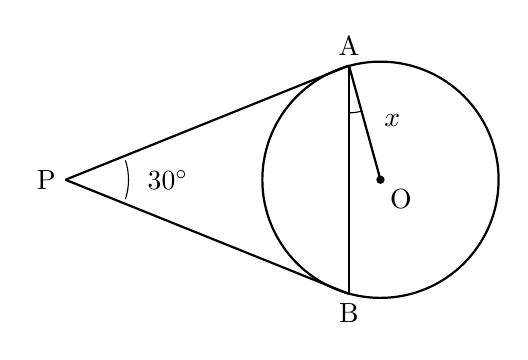
\begin{tikzpicture}[scale=1]

    % --- Coordinates ---
    % O is the center of the circle
    \coordinate (O) at (3,0);
    % P is the external point
    \coordinate (P) at (-1,0);
    
    % Points of tangency A and B (Calculated for geometric accuracy)
    \coordinate (A) at (2.6, 1.45);
    \coordinate (B) at (2.6, -1.45);

    % --- Circle ---
    % Drawing the circle with center O and marking the center dot
    \draw[thick] (O) circle (1.5);
    \fill (O) circle (1.5pt); 

    % --- Tangents and Geometric Lines ---
    \draw[thick] (P) -- (A); % Tangent line PA
    \draw[thick] (P) -- (B); % Tangent line PB
    \draw[thick] (A) -- (B); % Vertical chord AB
    \draw[thick] (A) -- (O); % Slanted radius OA

    % --- Arcs and Repositioned Text ---
    
    % Angle sign at vertex P for 30 degrees
    \draw (P) ++(18:0.8) arc (18:-18:0.8);
    \node at (0.3, 0) {$30^{\circ}$};

    % FIXED ANGLE SIGN AT A: Between chord AB and radius OA
    % Spanning from -90 degrees (downward) to -75 degrees (along radius)
    \draw (A) ++(-90:0.6) arc (-90:-73:0.6);
    
    % FIXED TEXT X: Moved further to the right for clarity
    \node at (3.15, 0.75) {$x$};

    % --- Point Labels ---
    % Placed to match Figure 11 exactly
    \node[left] at (P) {P};
    \node[above] at (A) {A};
    \node[below] at (B) {B};
    \node[below right] at (O) {O};

\end{tikzpicture}